% ****** Start of file apssamp.tex ******
%
%   This file is part of the APS files in the REVTeX 4.1 distribution.
%   Version 4.1r of REVTeX, August 2010
%
%   Copyright (c) 2009, 2010 The American Physical Society.
%
%   See the REVTeX 4 README file for restrictions and more information.
%
% TeX'ing this file requires that you have AMS-LaTeX 2.0 installed
% as well as the rest of the prerequisites for REVTeX 4.1
%
% See the REVTeX 4 README file
% It also requires running BibTeX. The commands are as follows:
%
%  1)  latex apssamp.tex
%  2)  bibtex apssamp
%  3)  latex apssamp.tex
%  4)  latex apssamp.tex
%
\documentclass[%
 reprint,
%superscriptaddress,
%groupedaddress,
%unsortedaddress,
%runinaddress,
%frontmatterverbose, 
%preprint,
%showpacs,preprintnumbers,
%nofootinbib,
%nobibnotes,
%bibnotes,
 amsmath,amssymb,
 aps,
%pra,
%prb,
%rmp,
%prstab,
%prstper,
%floatfix,
]{revtex4-1}

\usepackage{graphicx}% Include figure files
\usepackage{dcolumn}% Align table columns on decimal point
\usepackage{bm}% bold math
%\usepackage{hyperref}% add hypertext capabilities
%\usepackage[mathlines]{lineno}%  Enable numbering of text and display math
%\linenumbers\relax % Commence numbering lines

%\usepackage[showframe,%Uncomment any one of the following lines to test 
%%scale=0.7, marginratio={1:1, 2:3}, ignoreall,% default settings
%%text={7in,10in},centering,
%%margin=1.5in,
%%total={6.5in,8.75in}, top=1.2in, left=0.9in, includefoot,
%%height=10in,a5paper,hmargin={3cm,0.8in},
%]{geometry}
\usepackage{acronym}
\usepackage{eurosym}
\usepackage{bbding}  %checkmark symbols
\usepackage{rotating} %Rotate headers
\usepackage{array}
\usepackage{adjustbox}
\usepackage{xspace} 
\usepackage[table]{xcolor} %color 

%fancy table formatings
 \newcolumntype{R}[2]{%              
     >{\adjustbox{angle=#1,lap=\width-(#2)}\bgroup}%
     l%
     <{\egroup}%
 }
\newcommand*\rot{\multicolumn{1}{R{60}{1em}}}% no optional argument here, please!
\newcolumntype{C}[1]{>{\centering\let\newline\\\arraybackslash\hspace{0pt}}m{#1}}

%ednotes
\newif\ifEdNotes \EdNotestrue
\def\noednotes{\EdNotesfalse}
\def\ednotes{\EdNotestrue}
\newcommand{\doednote}[1]{{\color{red}(\textbf{Ed:} \textit{#1)}}}
\newcommand{\ednote}[1]{\ifEdNotes 
  \doednote{#1} 
\fi}

\newcommand{\epem}{\mbox{${\rm e}^+{\rm e}^-$}}


\begin{document}

\preprint{LCCPEB---}

\title{The International Linear Collider\\ An European Perspective}% Force line breaks with \\
\thanks{Version 1.3}%

\author{Juan Fuster}
% \altaffiliation[Also at ]{Physics Department, XYZ University.}%Lines break automatically or can be forced with \\
\author{et.al.}%
 \email{Second.Author@institution.edu}
\affiliation{%
 Authors' institution and/or address\\
% This line break forced with \textbackslash\textbackslash
}%

\collaboration{LCC Collaboration}%\noaffiliation

\date{\today}% It is always \today, today,
             %  but any date may be explicitly specified

\begin{abstract}
Input from the International Linear Collider community for the European Strategy Update

\end{abstract}

\pacs{Valid PACS appear here}% PACS, the Physics and Astronomy
                             % Classification Scheme.
%\keywords{Suggested keywords}%Use showkeys class option if keyword
                              %display desired
\maketitle

%\tableofcontents

\section{\label{sec:intro}Introduction}
Somewhere in intro: \\
This report uses the same steps and timelines as the KEK ILC action plan~\cite{kekactionplan}:
\begin{description}
\item[\bfseries 2017--2018: Pre-preparation phase] 
The on-going and recent activities with relevance to the ILC in Europe are reviewed for accelerators and detectors.
\item[\bfseries 2019--2022: Preparation phase]
This period needs to be initiated by a positive statement from the Japanese government about hosting the ILC, followed by a European strategy update that ranks European participation in the ILC as a high-priority item. The preparation phase focuses on preparation for construction and agreement on the definition of deliverables and their allocation to regions. The European groups will concentrate on preparation for their deliverables including working with and preparing European industry. Europe and European scientists, as part of an international project team, will also participate in the overall finalisation of the design, while in parallel contributing to the work of setting up the overall structure and governance of the ILC project and of the associated laboratory.
\item[\bfseries 2023 and beyond: Construction phase]
The construction phase will start after the ILC laboratory has been established and inter- governmental agreements are in place. At the current stage, only the existing capabilities of the European groups relevant for this phase can be described. As mentioned above, the detailed contributions will have to be defined during the preparation phase and formalised by inter-governmental agreements. 
\end{description}

With the completion of the foreseen nine-year construction phase in 2032, the European groups will naturally be involved in the commissioning of both the accelerator and detectors. \\
Steinar, Jim, Juan, 1.5 pages

\section{\label{sec:acc}Accelerator}

Europe has a very strong scientific, technological and industrial basis to make significant contributions to the construction of virtually 
any part of the ILC accelerator. In following three subsections the past/current activities, the ILC preparation phase and the subsequent construction phase 
will be described, from the perspective of European capabilities for and participation in constructing the ILC accelerator. 
A final subsection considers the organisation of the future ILC accelerator activities on the European side. 

\subsection{ILC accelerator competence in Europe~\label{sec:acc:competence}}

The key recent and ongoing activities in Europe with high relevance for ILC are the direct
European participation in the ILC Global Design Effort (GDE) and the Linear Collider Collaboration (LCC),
the European XFEL (E-XFEL) project at DESY , the European Spallation Source (ESS) superconducting linac, the European 
participation in the ATF-2~\cite{Grishanov:2005ek,Grishanov:2006kx} at KEK for linear collider studies, the E-JADE Marie 
Curie project~\cite{ejade}, and the CLIC study~\cite{Aicheler:2012bya,Linssen:2012hp}. The following paragraphs 
will summarize these briefly, while a more comprehensive description can be found in ~\cite{ejade-report}. \ednote{ALL THESE NEED DEFINITION AND REFS - UNDERWAY}

During 2007-2012 the ILC GDE was responsible for the coordination of the worldwide ILC accelerator design. 
R\&D and cost-estimate development during this period culminated in the publication of the ILC Technical Design Report in 2013~\cite{Behnke:2013xla}. 
The estimated European FTE contributions (728 person years in total) during 2007-2012 is summarised in Figure~\ref{fig:PrePrep:ilcgde4}, 
divided into accelerator domain issues and SCRF technology development (excluding management and documentation support). 
Note that the SCRF numbers represent ILC-specific resources and do not include the extensive synergetic contributions from the European XFEL.

\begin{figure}[htbp]
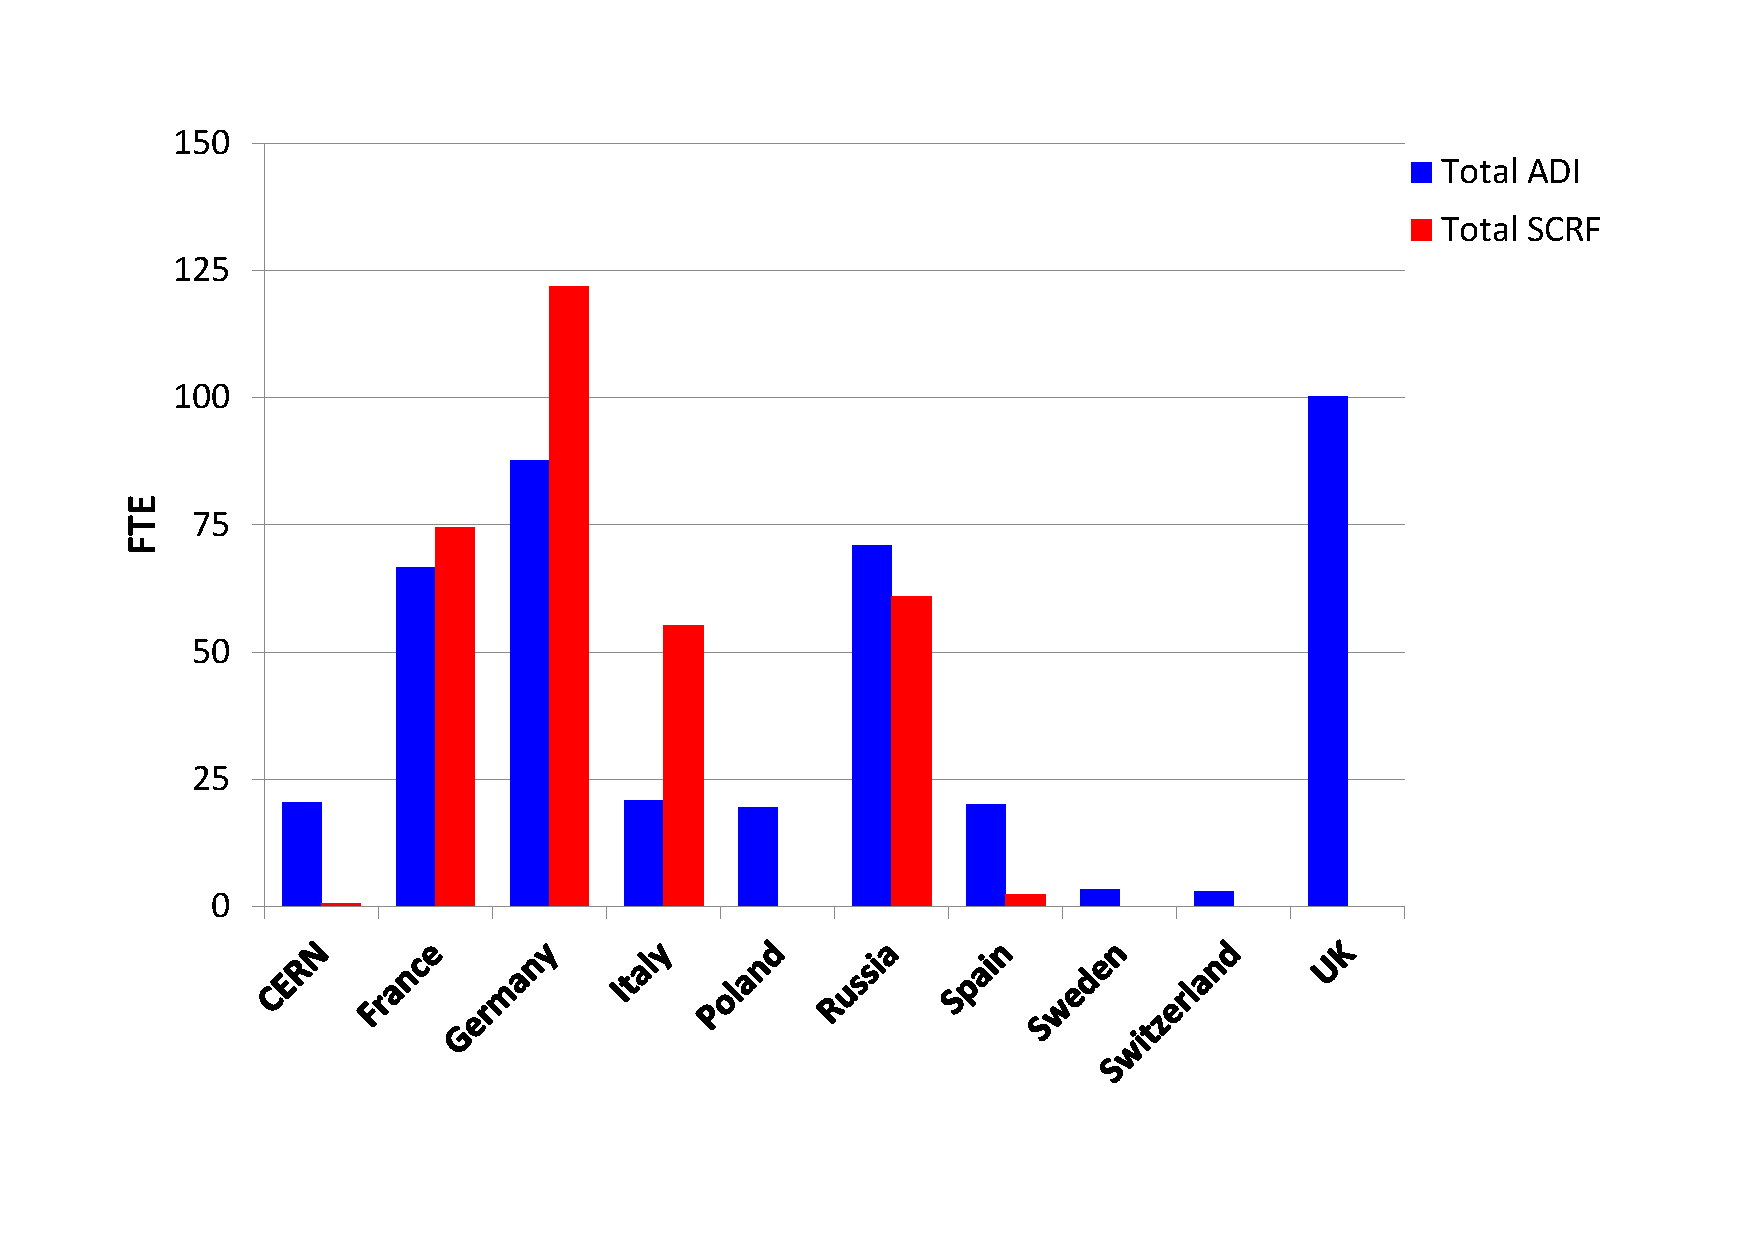
\includegraphics[width=0.45\textwidth]{figures/EU-GDE-FTE-columns-per-country.pdf}
\caption{\label{fig:PrePrep:ilcgde4} The contribution to the ILC GDE (2007-2012) in staff years per European country, separately for SCRF and accelerator domain studies (ADI).}
\end{figure}

%\vspace{0.15cm}
After the delivery of the ILC TDR in 2013, the European SCRF expertise moved fully into construction of the European XFEL at DESY (discussed in next paragraph). 
The GDE was replaced by the LCC. In spite of limited direct funding for ILC studies in Europe the combined efforts in 
several related projects have allowed European researchers to continue activities in the framework of the LCC, in close collaboration with Japan, during
the last five years. These were to a large degree focused on studies for implementing a 250~GeV ILC machine in Japan. 
These European activities are as follows:
\begin{itemize}
\item Participation in the LCC Accelerator Design and Integration (SCRF, Cryogenics, High-Level RF (HLRF), Civil Engineering, Beam dump, Positron source, Radiation safety)
\item Participation in the ATF-2 programme at KEK (nano beams and final focus)
\item Combined studies with CLIC in several areas (beam-dynamics, modelling/simulation, damping rings, RTML, Beam Delivery System(BDS), Machine-Detector Interface (MDI), cost and power)
\item E-JADE supported secondments of European researchers to Japan for ILC and ATF-2 related activities.
\end{itemize}
These activities involves groups in Spain, France, DESY, UK, Italy and CERN. 

%Table~\ref{fig:PrePrep:gdelccadi}. 

%\begin{table}[htbp]
%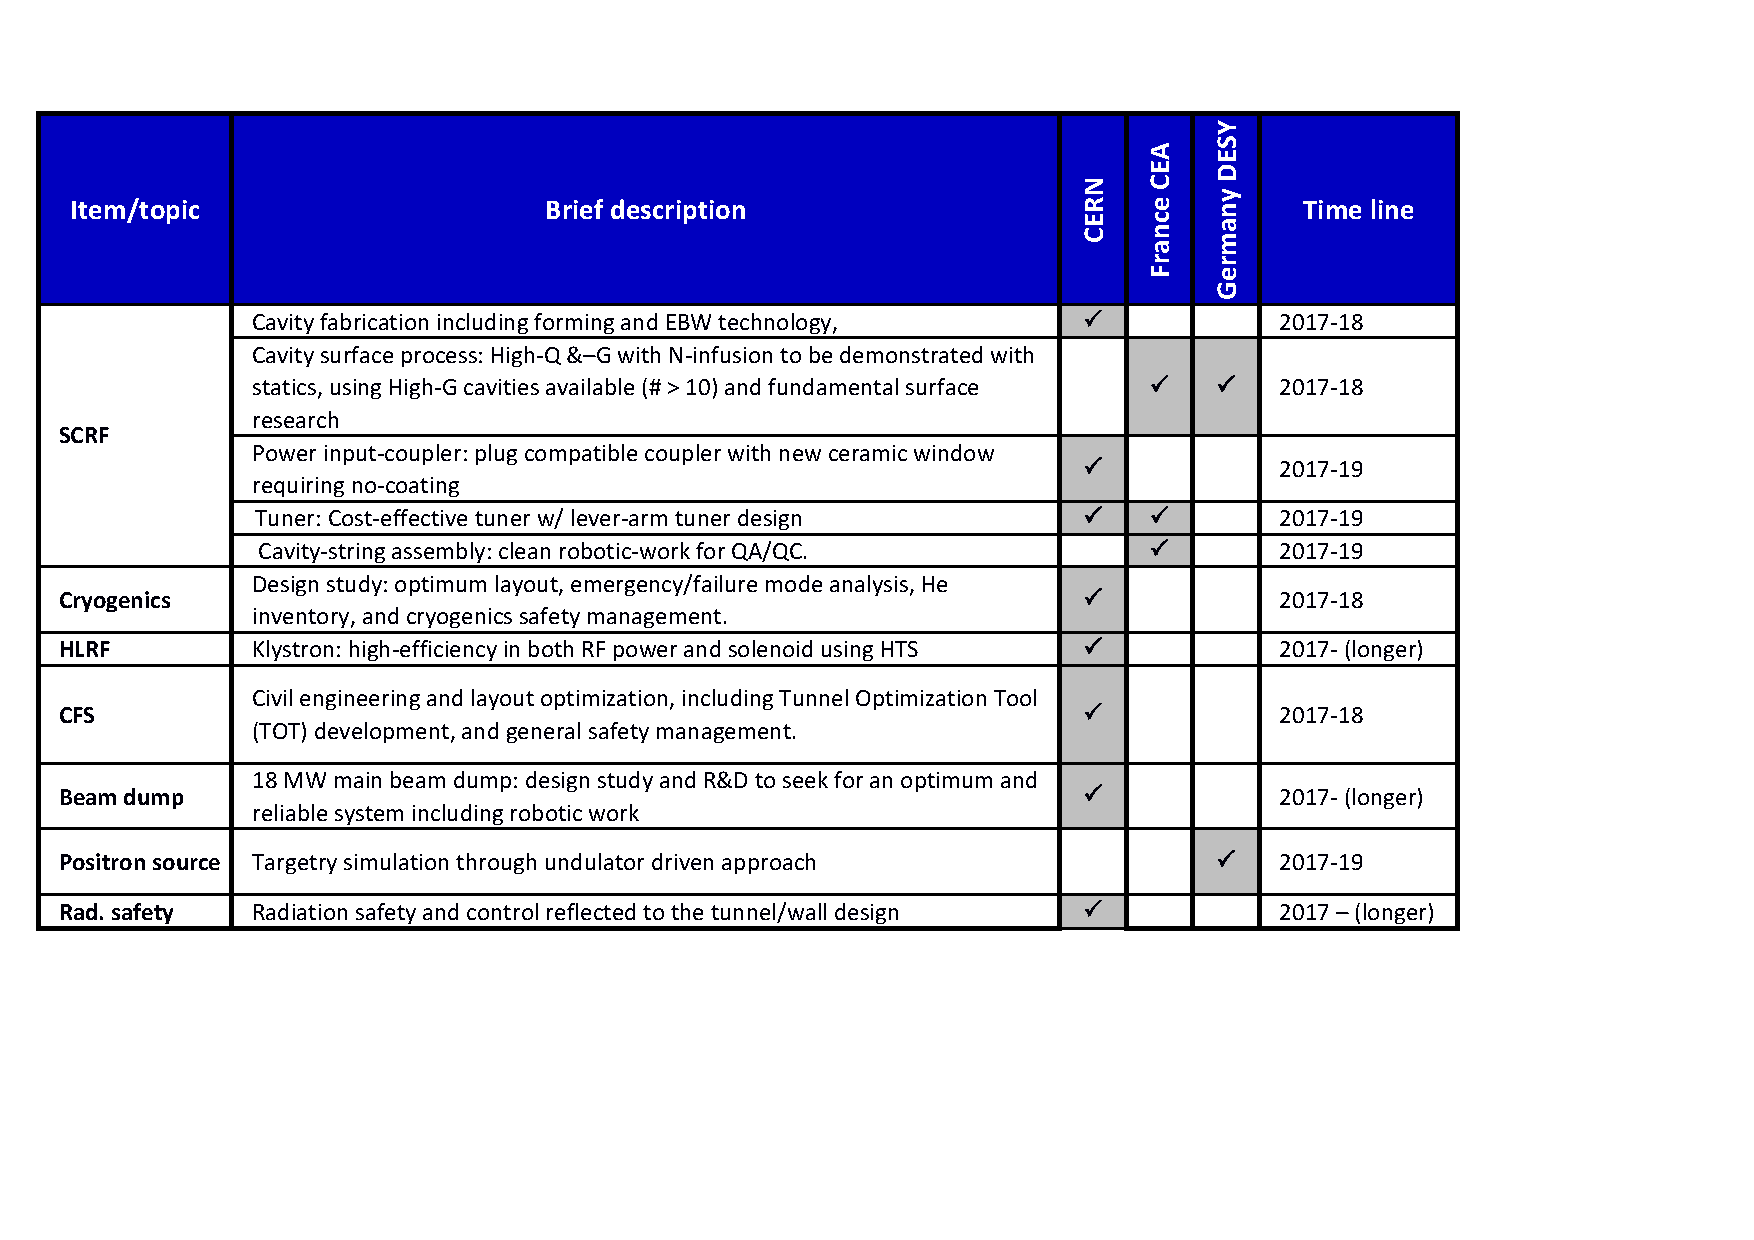
\includegraphics[width=0.45\textwidth]{figures/ILCEAP-Matrices-LCCADI.pdf}
%\%caption{\label{fig:PrePrep:gdelccadi} Current and recent common studies between European institutions and Japan relevant for the ILC in the framework of LCC (revise with Akira). In parallel several European groups have played leading role in the ATF-2 programme at KEK for linear collider nanobeam and final focus students, involving students and researchers from France, Spain, UK, CERN and DESY.}
%\end{table}

Beyond the activities described above, the European XFEL project at DESY is nevertheless the most prominent example of European capabilities for contributing to construction of the ILC accelerator.
The 17.5~GeV superconducting linac at the E-XFEL at DESY, comprises 100 superconducting ILC-like cryomodules (800 1.3~GHz TESLA cavities) driven by 25 10~MW multibeam klystrons. The E-XFEL linac configuration is very similar to that foreseen for the ILC and can be seen as a 7\% (in energy) ILC prototype. The cryomodules were produced by a consortium of six European countries together with predominantly European industries. The consortium members and the various responsibilities across the linac-relevant E-XFEL work packages (including testing) are given in Table~\ref{tab:acc:XFELResponsibilities}.

% \begin{table*}[t]
% 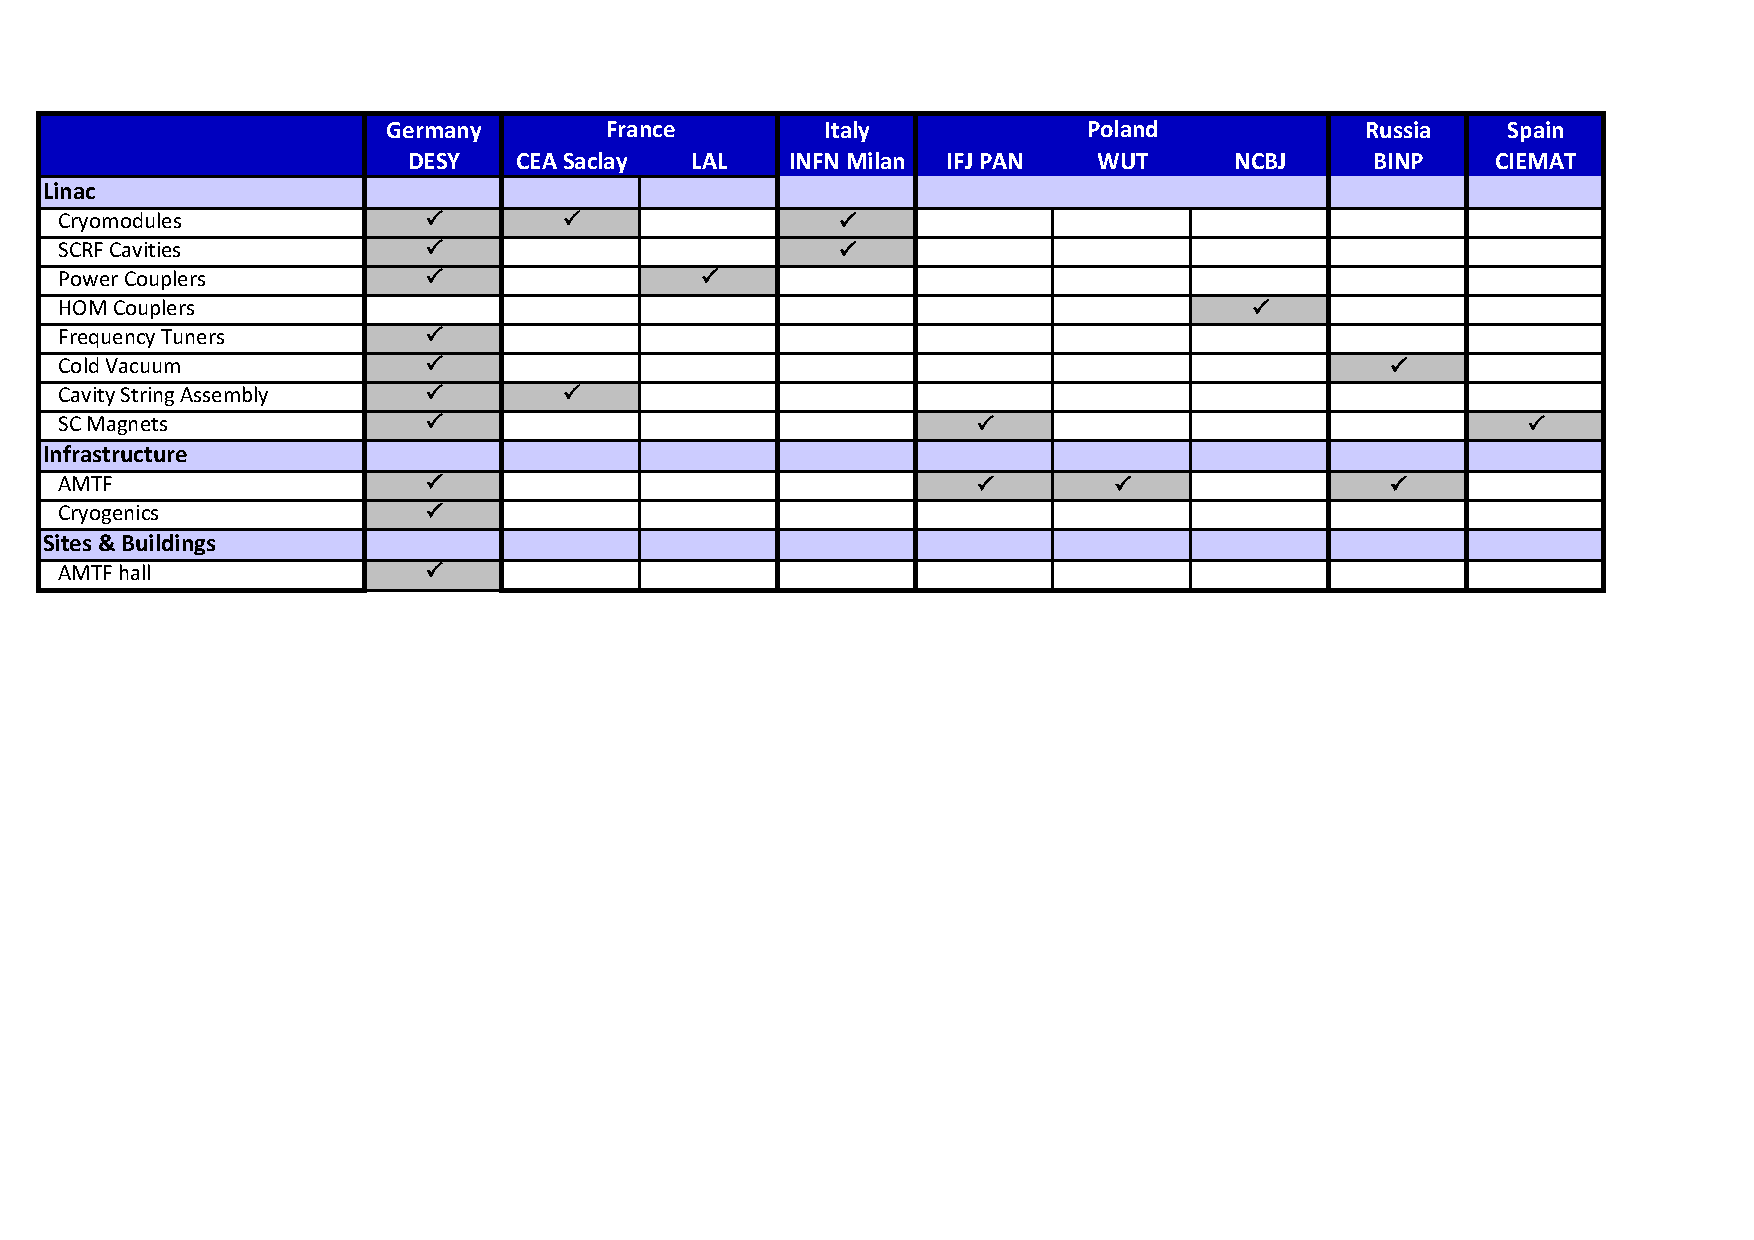
\includegraphics[width=\textwidth]{figures/ILCEAP-Matrices-XFEL.pdf}
% \caption{\label{tab:PrePrep:XFELResponsibilities2} Responsibility matrix for cryomodule production and testing for the European XFEL.} 
% \end{table*}

\begin{table}[htbp]
\begin{tabular}{l|C{0.6cm}|C{0.6cm}|C{0.6cm}|C{0.6cm}|C{0.6cm}|C{0.6cm}|}

	& \rot{\bfseries Germany}& \rot{\bfseries France}&\rot{\bfseries Italy}&\rot{\bfseries Poland}&\rot{\bfseries Russia}&\rot{\bfseries Spain} \\\hline
\bfseries Linac&&&&&&\\[5pt]\hline
\hspace{0.3cm}Cryomodules		&\Checkmark&\Checkmark&\Checkmark&&&\\[5pt]
\hspace{0.3cm}SCRF Cavities		&\Checkmark&&\Checkmark&&&\\[5pt]
\hspace{0.3cm}Couplers and Tuners	&\Checkmark&\Checkmark&&\Checkmark&&\\[5pt]
\hspace{0.3cm}Cold Vacuum		&\Checkmark&&&&\Checkmark&\\[5pt]
\hspace{0.3cm}Cavity String Assembly	&\Checkmark&\Checkmark&&&&\\[5pt]
\hspace{0.3cm}SC Magnets		&\Checkmark&&&\Checkmark&&\Checkmark\\[5pt]\hline
\bfseries Infrastructure&&&&&&\\[5pt]\hline
\hspace{0.3cm}AMTF			&\Checkmark&&&\Checkmark&\Checkmark&\\[5pt]
\hspace{0.3cm}Cryogenics		&\Checkmark&&&&&\\[5pt]\hline
\bfseries Sites \& Buildings&&&&&&\\[5pt]\hline
\hspace{0.3cm}AMTF hall		&\Checkmark&&&&&\\[5pt] \hline
\end{tabular}

\caption{\label{tab:acc:XFELResponsibilities} Responsibility matrix for cryomodule production and testing for the European XFEL. 
More details and a similar matrix can be found in ~\cite{ejade-report} concerning construction of SCRF modules for the ESS. 
The latter also includes Sweden and UK as well as new groups in several of the countries already involved in the E-XFEL construction. 
The ESS effort is also strategically important for ILC as infrastructures and industries are being updated and procedures are improving also today.} 
\end{table}

Construction of the European XFEL is now complete, and the SCRF linac has been brought into operation. The E-XFEL can directly benefit the ILC in several ways: 
\begin{itemize}
\item The experience and knowledge gained during the unprecedented industrial
production of 100 cryomodules over a three-year period can provide 
invaluable input to any future large-scale production for the ILC. The detailed cost breakdown of the E-XFEL cryomodules 
provides a solid basis for any future projection of a possible European in-kind contribution to the ILC. 
\item 
The currently ongoing commissioning of the E-XFEL and its future operation will provide invaluable ``system testing'' for the ILC, 
including understanding the ultimate performance of the modules with beam loading, beam control (LLRF development), software tools, 
and more general operational experience. 
\item The infrastructure that was constructed for E-XFEL cavity and module 
testing, high-power coupler conditioning and module assembly will continue to be maintained, and (in the case of the testing infrastructure) will provide a significant support for SCRF R\&D.
\end{itemize}

The expertise and infrastructures established for the E-XFEL are now deployed in the construction of SCRF modules for the ESS. 
The consortium is slightly different with Sweden and UK joining, DESY for obvious reasons less involved, and several new groups from countries already 
involved in the E-XFEL. The ESS effort is also strategically important for ILC as it ensures that infrastructures and industries 
are being updated and procedures are improving also today.

\subsection{ILC accelerator preparation phase activities in Europe ~\label{sec:acc:prephase}}

The overall resources needed during the four-year preparation phase are estimated to be 5\% of the material and 10\% of the personnel 
foreseen for the initial 250~GeV accelerator project construction. Irrespective of the final level of European investment into the ILC, 
and to allow the preparation phase to begin after an official expression of interest from Japan and support by the European strategy, 
it would be appropriate that, given its expertise and previous involvement, Europe invests 1/3 of the overall effort required in the 
preparation phase. The remainder of this section assumes this to be the case. This would then amount to a total European material 
budget of 85 M\euro{} and 240 FTE-years, integrated over the period.
Distributed over four years, an average yearly budget of around 30 M\euro{} (covering material and personnel) would be needed with an 
increasing profile from 2019 towards 2022. The resources required for the activities in the preparation phase are hence similar in 
scope to those used by existing project studies such as CLIC and FCC. One important difference will be that the ILC preparation 
requires a strong engineering team, such that the profile of the ILC personnel will be towards more engineering and technical 
design and gradually less focused on R\&D studies.

The preparation phase will be used for three main purposes:

\begin{itemize}
\item 
Technical preparation of the major European deliverables foreseen for the construction phase. 
This covers final technical specifications, final prototypes, the preparation of pre-series orders and the preparation of local 
facilities. A particularly important point for Europe is the transfer of European XFEL know-how and the preparation of the 
relevant facilities for ILC construction.
\item
The other key technical activity will be the organisation of a strong European design office for ILC that will liaise with 
other such offices: there will certainly be a host-lab office in Japan, but additional international design offices will be 
required. In Europe, the installation of a central European Design Office at CERN with satellite offices in other European laboratories is considered the most viable model.
\item 
The third key activity in the preparation phase will be negotiations about the final European ILC contributions, about the 
organisation of the project in the construction and operation phase, and about a future governance model for the ILC. These issues are discussed in further chapters of this document.
\end{itemize}

The key activities are summarised in table~\ref{fig:prep-phase-summary} - unify format.


% \begin{table}[htbp]
% 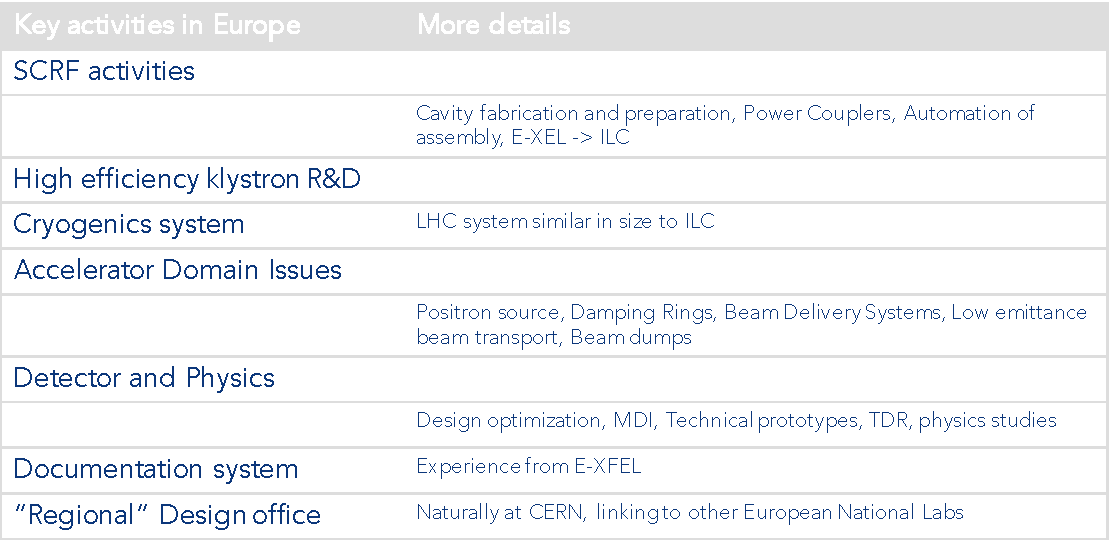
\includegraphics[width=0.45\textwidth]{figures/prep-phase-summary.pdf}
% \caption{\label{fig:prep-phase-summary2} Key activities during the preparation phase}
% \end{table}


\begin{table}[htbp]
\begin{ruledtabular}
\begin{tabular}{p{3.5cm}p{4.75cm}}
 \bfseries {Activities in Europe} &\bfseries{More details}                                                         \\
SCRF activities			&Cavity fabrication and preparation, Power Couplers, Automation of assembly, European XFEL $\rightarrow$ ILC\\
High efficiency klystron R\&D   &Reaching 70\% efficiency or above with several vendors   \\
Cryogenics system               &LHC system similar in size to ILC\\
Accelerator Domain Issues       &Positron source, Damping Rings, Beam Delivery Systems, Low emittance beam transport, Beam dumps\\
Detector and Physics            &Design optimization, MDI, Technical prototypes, TDR, physics studies\\
Documentation system            &Experience from E-XFEL                                       \\
“Regional” Design office        &Naturally at CERN, linking to other European National Labs \\
\end{tabular}
\end{ruledtabular}
\caption{\label{fig:prep-phase-summary} Key activities during the preparation phase}
\end{table}


\subsection{ILC accelerator in-kind contributions from Europe ~\label{sec:acc:constrphase}}

The actual contribution from Europe will be determined by negotiations at a 
later stage, and no formal commitments can be made at this time. The models 
chosen for in-kind contributions in this document, and discussed in this 
section, are as follows: Europe — being one of three major regions involved in 
the ILC project delivers 1/3 of the non-CFS (civil engineering and conventional facilities) 
components of the ILC accelerator. The CFS work 
and components will naturally be constructed in — and installed and 
commissioned by — the host nation. The models follow recommendations given in 
the Nomura report~\cite{Nomura-eng} and are also drawn from the ILC Project Implementation 
Planning (PIP) document~\cite{ILCPIP}. The models discussed correspond to an overall 
European contribution of around \ednote{\bfseries ??\%} to the ILC accelerator project. 

\begin{figure}[htbp]
\begin{center}
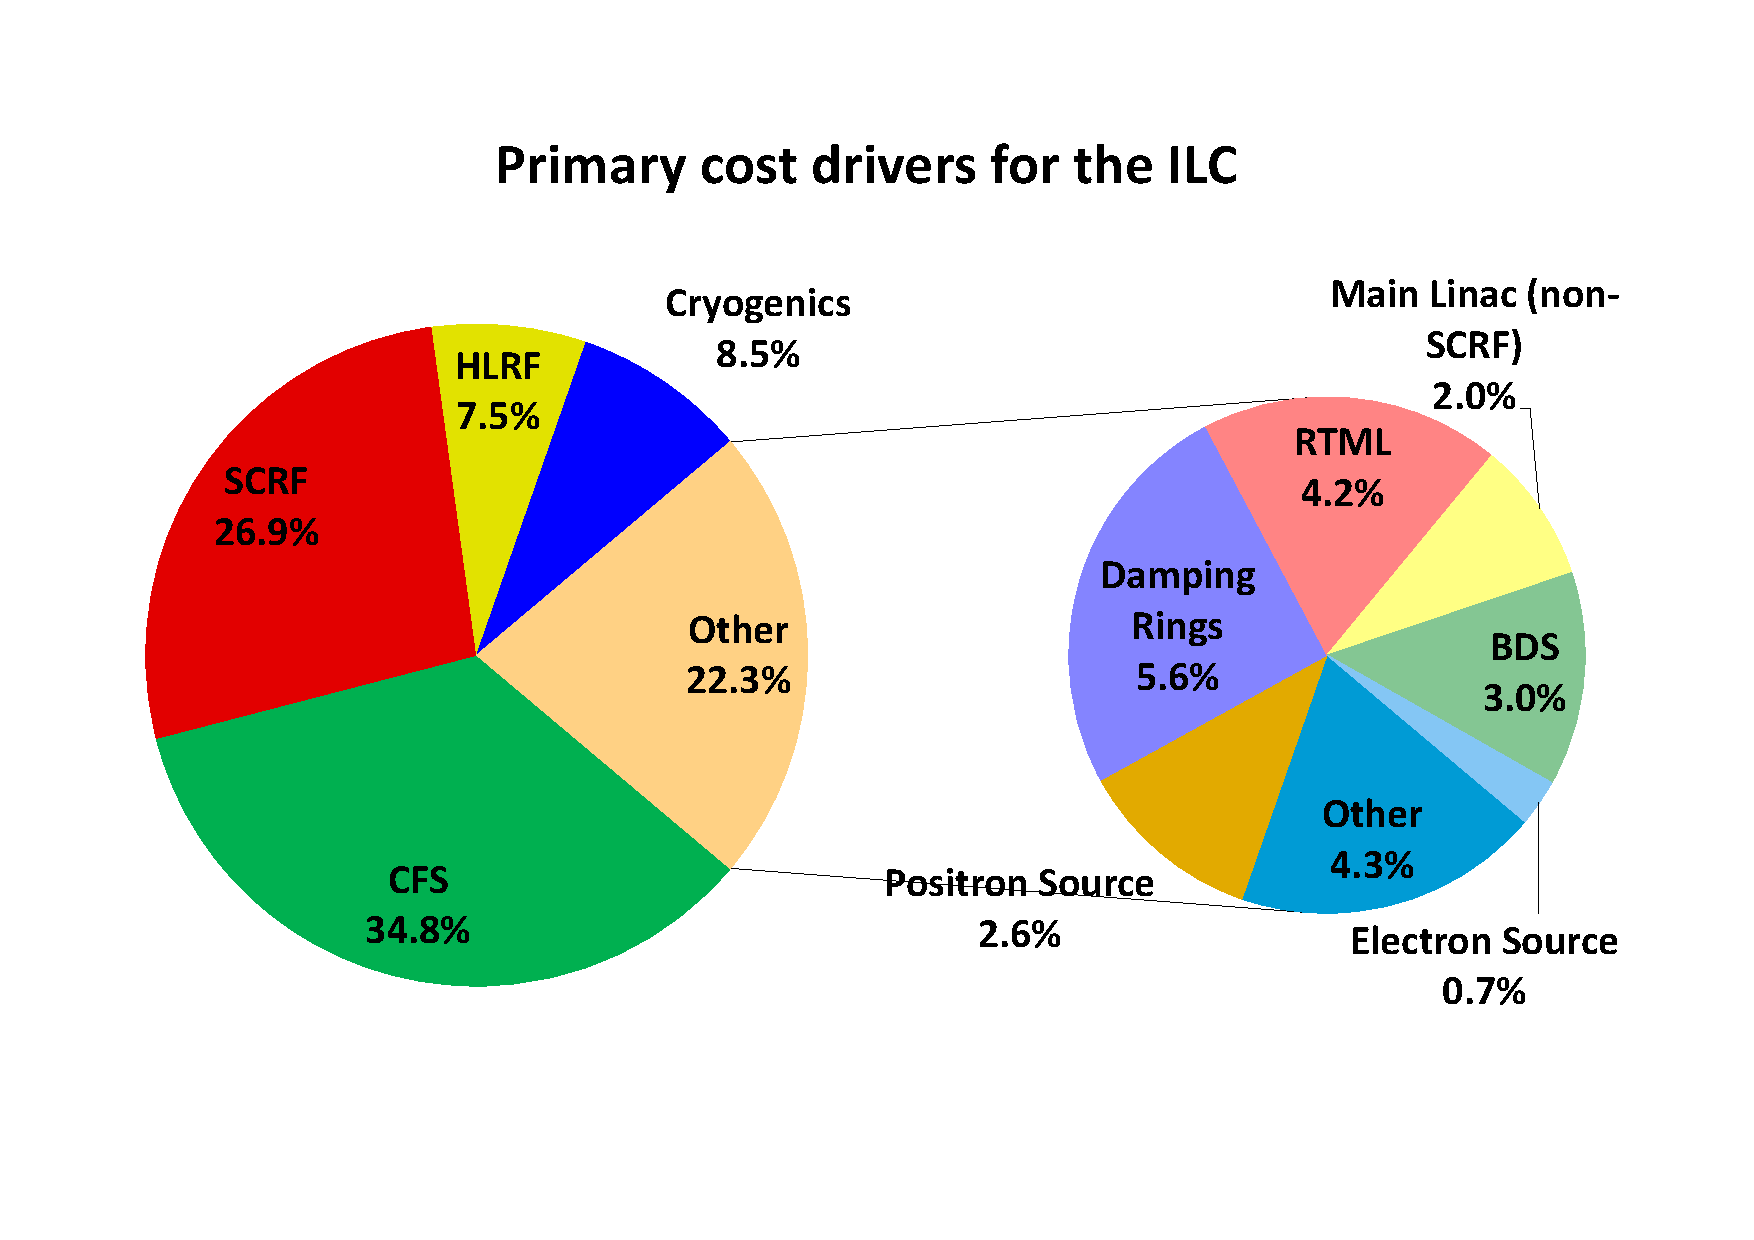
\includegraphics[width=0.48\textwidth]{figures/eap-chp3-ilccostdrivers.pdf}
 \caption{\label{fig:constructionmodel:ILCPrimaryCostDrivers} Primary cost drivers for the ILC (breakdown based on ILCU). \ednote{Needs Update to 250 GeV}}
\end{center}
\end{figure}

Figure~\ref{fig:constructionmodel:ILCPrimaryCostDrivers} shows the primary cost drivers of the ILC as identified in the TDR~\cite{Adolphsen:2013kya}. The dominant cost driver is the production of approximately 930 SCRF cryomodules. Given European expertise, 
existing infrastructure, and proven industrial capability arising from the construction 
of the E-XFEL and ESS, it is widely assumed that a large fraction of the European in-kind contribution 
will be in the form of cryomodules. The ILC TDR assumed that three, possibly four, production sites 
would be required worldwide. 
The European XFEL has been constructed by a consortium of several European countries, with DESY providing overall coordination. Based on this experience and the known published cost of the E-XFEL cryomodules, we have produced a model for producing and testing one-third of the cryomodule production (310 cryomodules). This model has then been used to scale to other possible contribution scenarios discussed below.The resulting cost per cryomodule is about 1.56 M\euro{} (material and labour), including module production and 100\% testing of cavities and cryomodules, which represents an approximate reduction of 30\% over the actual E-XFEL cost. This reduction has been estimated through the higher production numbers and the re-use of existing E-XFEL production and testing infrastructure.  Where applicable, a mild learning curve slope of 95\% has been applied, assuming two vendors for procurement of all major sub components. \ednote{REVISE NOW WITH LOWER NUMBER}.

Europe not only has expertise in cryomodule production, but also in many other 
of the subsystems required for the ILC. A European contribution to ILC could 
also include other items in addition to cryomodules. As an example, providing 
one third of the klystrons, modulators and associated controls (low-level RF) 
needed for the SCRF linacs would cost around 280~M\euro{}, one third of the cost of 
the cryogenics systems would be roughly 210~M\euro{}, and supplying a fraction of the 
accelerator components (vacuum, power supplies, magnets, computing and controls 
etc.) needed for the project could easily reach a cost of approximately 350~M\euro{}. 
Figure~\ref{fig:constructionmodel:ILCPrimaryCostDrivers} shows the ILC TDR costs broken down by both accelerator sub-system and 
technical components, not including CFS, installation or SCRF cryomodules.

\ednote{Discuss European matrix (TABLE 3).}

\begin{table*}
\begin{tabular}{l|C{1.8cm}|C{1.8cm}|C{1.8cm}|C{1.8cm}|C{1.8cm}|C{1.8cm}|C{1.8cm}|C{1.8cm}|}
 	&\bfseries SCRF	& \bfseries HLRF	&\bfseries Sources&\bfseries Damping Rings	&\bfseries Instru\-mentation&\bfseries Beam Dynamics	&\bfseries Beam Delivery System	&\bfseries Cryogenics \\\hline
CERN	&	&C,O	&O	&G,C,O		&C,G		&C,G		&C,G			&O\\
France	&X,E,G	&	&G	&		&A,G		&G		&C,G			&\\
Germany	&X,G	&	&G	&G		&		&G		&			&O\\
Italy	&X,E,G	&	&	&G		&		&		&			&\\
Poland	&X,E	&	&	&		&		&		&			&\\
Russia	&X	&	&G	&		&		&		&			&\\
Spain	&X,E	&	&	&		&A		&		&C,G			&\\
Sweden	&E	&	&	&		&		&		&G			&\\
Switzerland& 	&	&	&		&X,C		&		&			&\\
UK	&E	&	&G	&G		&A,C,G		&C,G,A		&C,G,A			&\\                                        \hline
\end{tabular}
\caption{The past European capabilities for the ILC accelerator construction. This is based on two major construction projects, the  E-XFEL (X) and the ESS (E),  
several more R\&D oriented efforts, the GDE/LCC (G), ATF-2 (A), CLIC and  experiences in other accelerator projects (O)}
\end{table*}


\ednote{Discuss profile (use figure included - needs re-check)}

As discussed in Section~\ref{sec:acc:prephase}, an assumed 5\% of the total value and 10\% of the personnel are assumed
to ramp up during the four-year preparatory phase. The profiles also includes a fraction
of the expected lab services personnel, which will almost certainly be required during this
phase. 

\begin{figure}[htbp]
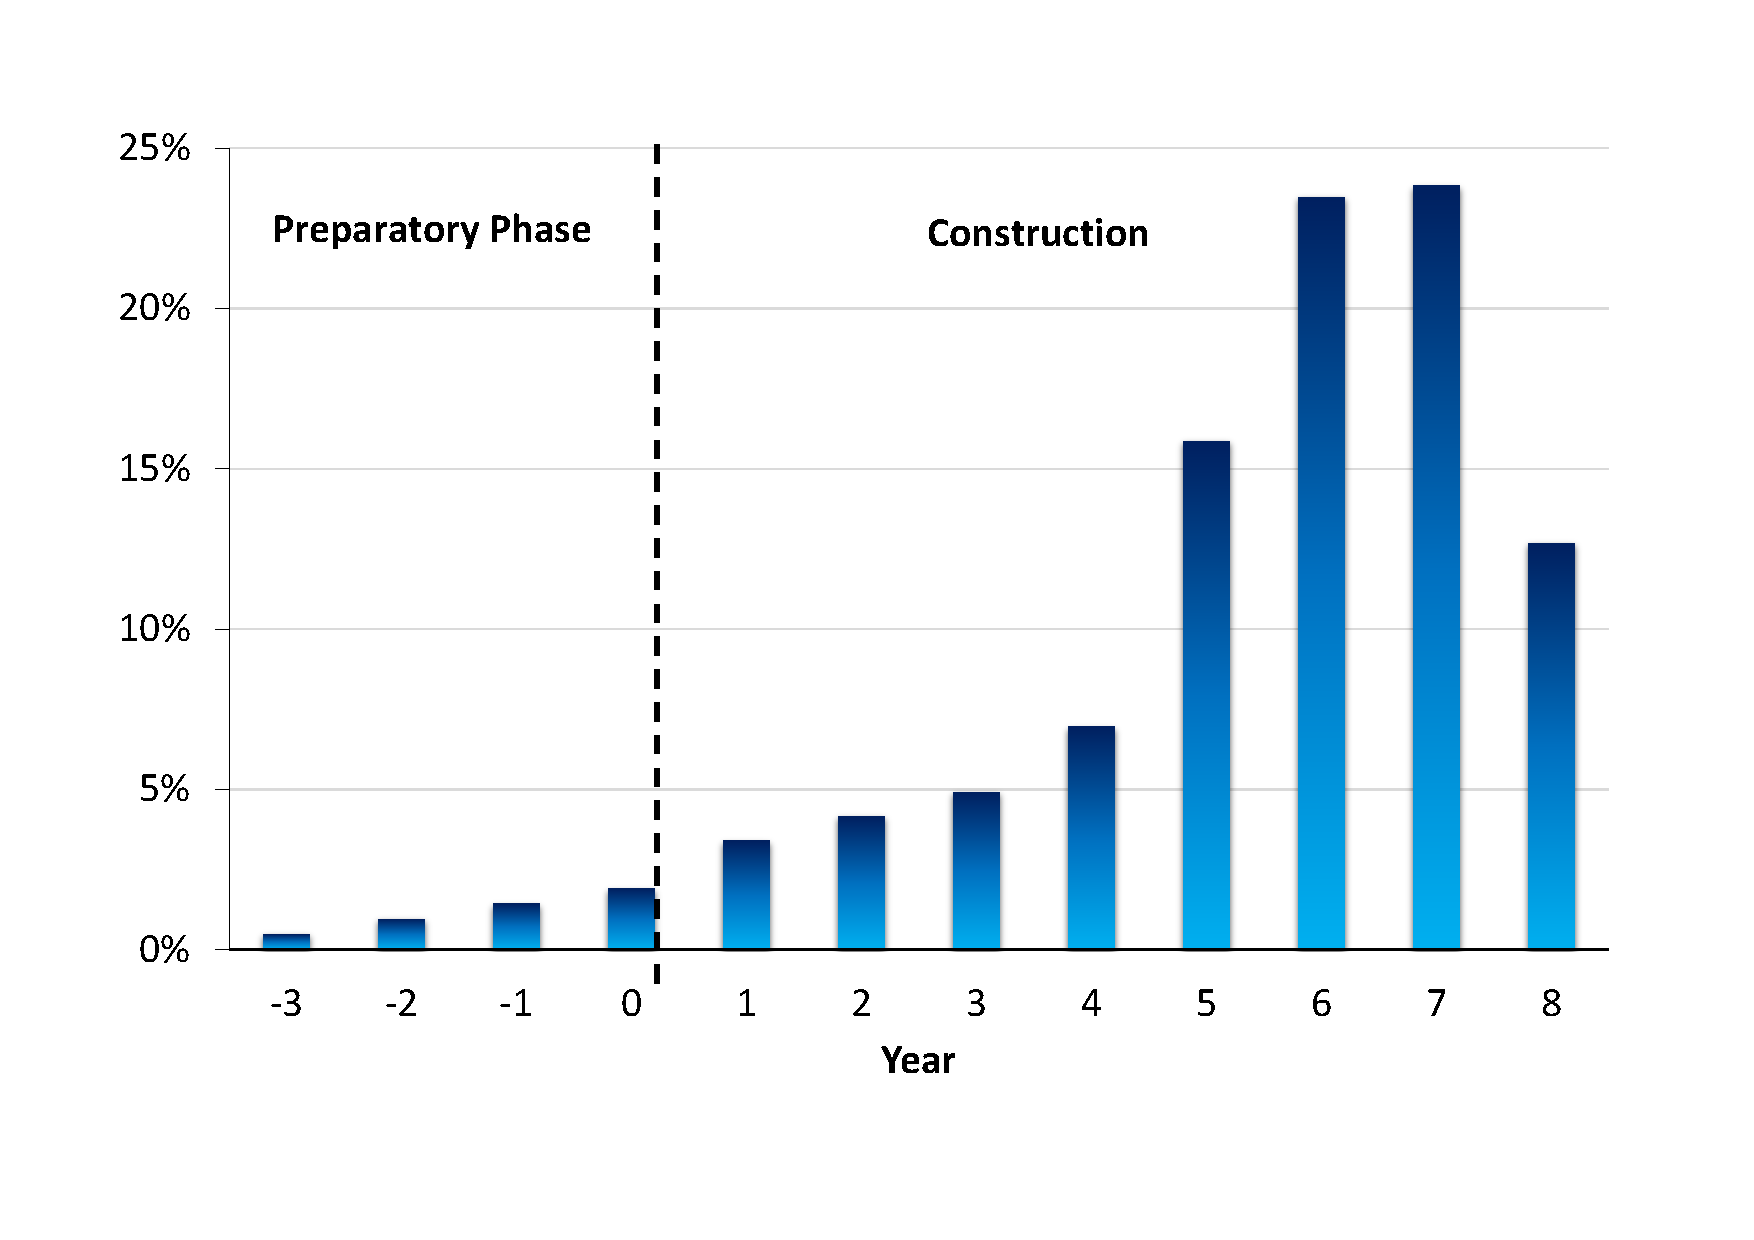
\includegraphics[width=0.475\textwidth]{figures/ilc-eu-ikc-cost-profile-blue-250me.pdf}
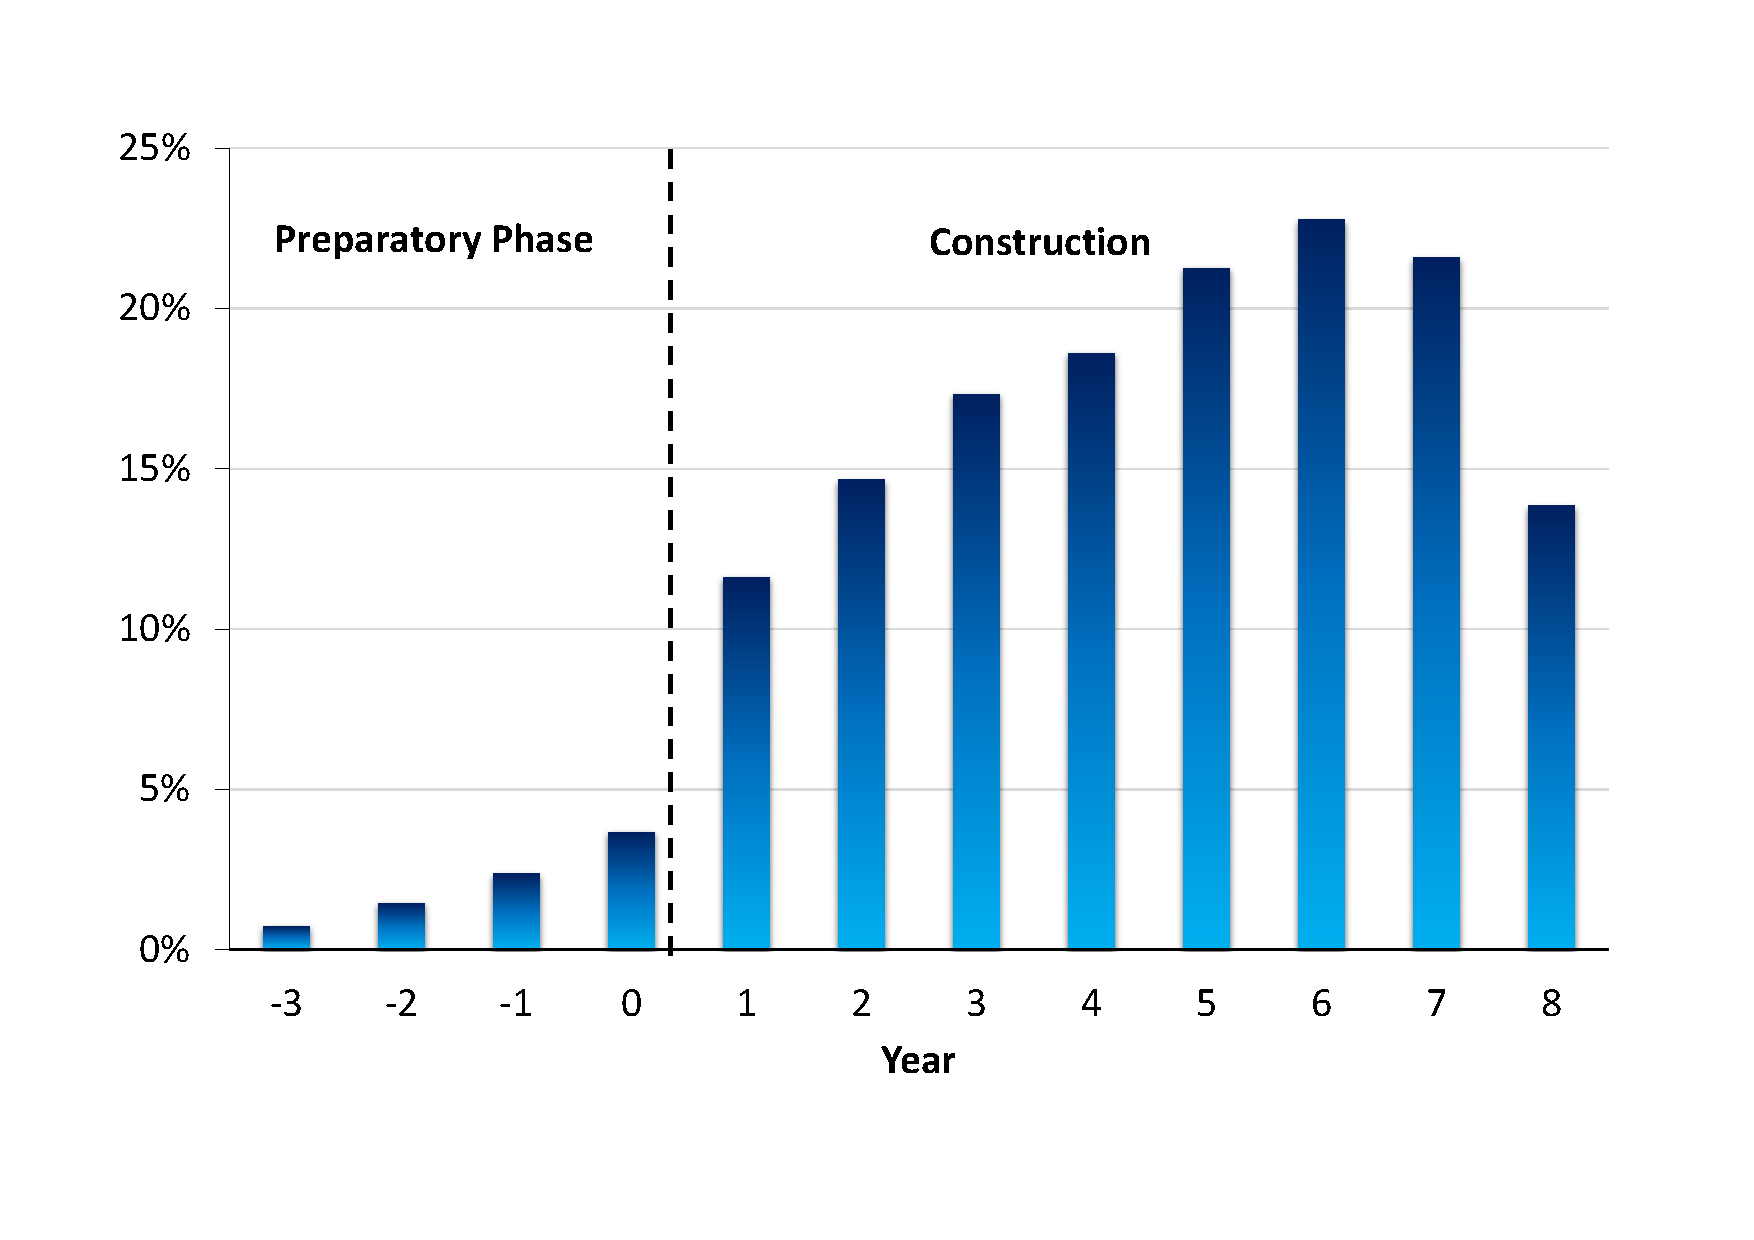
\includegraphics[width=0.475\textwidth]{figures/ilc-eu-ikc-cost-profile-blue-fte.pdf}
\caption{\label{fig:costprofile:costprofile} An estimation of the cost and personnel profile cover the preparatory phase (years -3 to 0) 
and the construction phase (years 1 to 8) for the 1/3 model of a 250~GeV machine, as a fraction of the
totals. In this timeline, 
year 1 corresponds to the first year of construction currently foreseen in 2023 
Top: capital costs. Bottom: explicit personnel in FTE.
}
\end{figure}


\subsection{\label{sec:acc:org}Organisation of the accelerator activities}
\ednote{[FROM EJADE REPORT - WRITE HERE ABOUT ACC.,  MOVE DET. PART TO III.D]}
In this short chapter we discuss possible organisation forms of a European 
participation in the ILC. 
On the accelerator side, the typical model is based on a leading host laboratory supported by 
bi-lateral agreements for in-kind deliverables from other funding agencies and 
laboratories. This was the model used during the LHC construction. 
The exact organisation of Europe's contribution to the ILC is not clear as of today 
and beyond the scope of this document. In any case, our current assumption is that 
CERN will play a leading role in the European participation in the ILC.

\ednote{Also from Action Plan}
Given the physics interests in a future \epem accelerator, the ILC project is likely to imply a substantial investment from
the European perspective. This fact highlights the necessity for a high-level
agreement about the level of European participation in ILC to be formalised between 2020
and 2023 if the currently assumed time-line of the ILC project is to be respected. Various
financing models for European contribution can be envisaged, including bilateral agreements
between Japan and European partners and models combining CERN resources with direct bilateral
agreements. The organisation of the European efforts towards a coherent contribution to ILC
from Europe, scientifically and technically with CERN in a leading coordinating role, seems to be
the most realistic and effective scenario.


\section{\label{sec:det}Detector}
\ednote{Marcel, Ties, 2 pages}

Detectors at colliding beam facilities are large international efforts, realised by strong collaborations. 
Typically many countries join forces, and contribute mostly in-kind to the building of the detector systems. 

Within the ILC project, the community has come together behind two complementary detector concepts, the SiD and the ILD detector concept. 
After a call for ``letters of intent'' in 2009~\cite{Aihara:2009ad,Abe:2010aa}, the two detector concept groups submitted their proposals 
which were validated and then presented in Volume 4 of the ILC TDR ~\cite{Behnke:2013lya}.

\subsection{ILC detector competence in Europe~\label{sec:det:competence}}
Europe has participated strongly in the work on the ILC detector concepts and 
related technological developments. Initiated by the TESLA project at the start 
of the century, an international effort was put into place to develop the needed 
detector technologies. This is augmented by strong national support, but also by 
European programs like the EUDET initiative (2006-2010), the AIDA program 
(2011-2015) or the AIDA-2020 program (2016-2019). In Europe, both CERN and DESY 
act as a hub of activity and provide common infrastructures and facilities 
including test beams. Programs in Asia, in particular in Japan, and in the 
Americas also played an important role in the ILC concepts. 

% \begin{table*}[t]
% 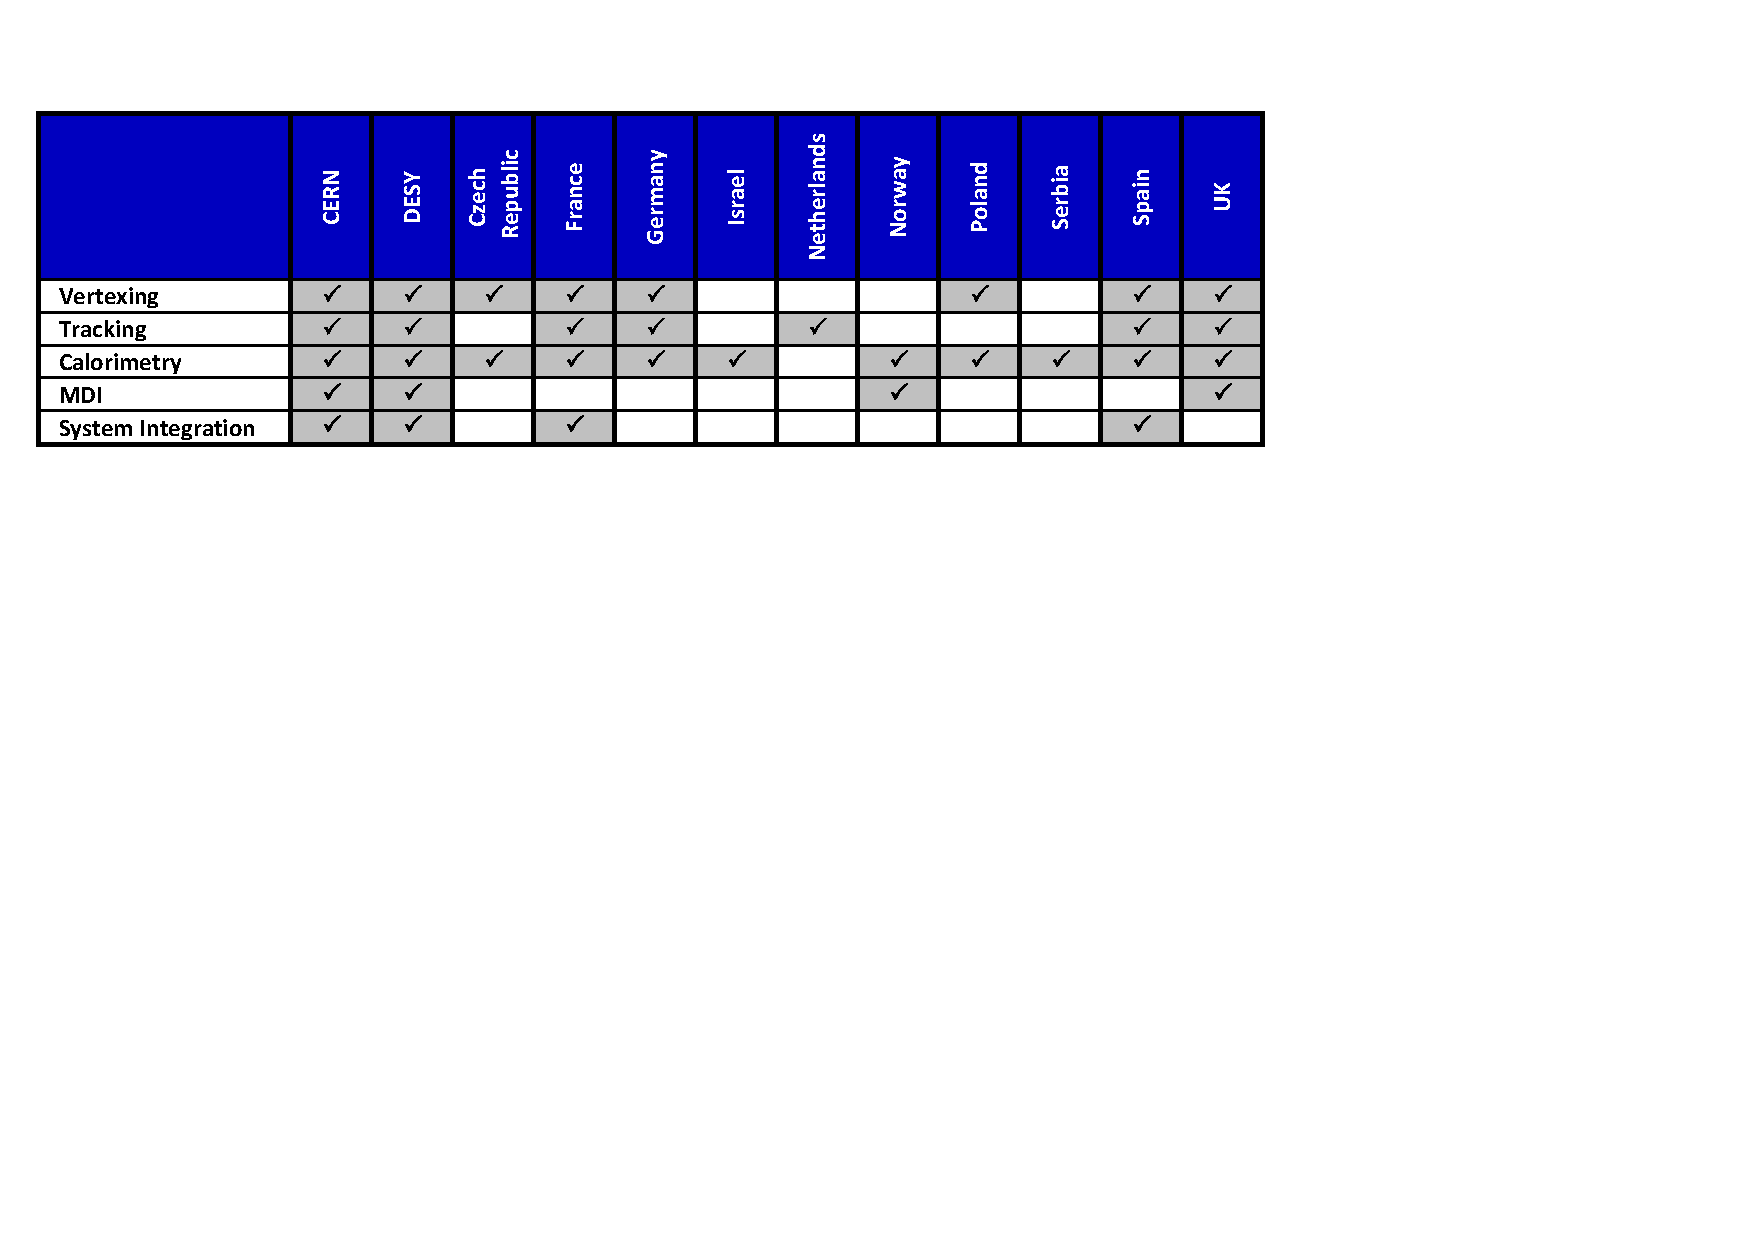
\includegraphics[width=\hsize]{figures/ILCEAP-Matrices-detectors.pdf}
% \caption{\label{tab:PrePrep:detectors} An overview of recent activities in the area of ILC-related detector R\&D and integration in Europe. \bfseries{Juan's Survey 2015, may need Updates}}
% \end{table*}

 \begin{table}[htbp]

\begin{tabular}{l |c |c |c |c |c |c |c |c |c |c |c |c|}
           &  \rot{ \bfseries CERN} & \rot{ \bfseries DESY} & \rot{ \bfseries Czech Republic} & \rot{ \bfseries France} & \rot{ \bfseries Germany} & \rot{ \bfseries Israel} & \rot{ \bfseries Netherlands} & \rot{ \bfseries Norway} & \rot{ \bfseries Poland} & \rot{ \bfseries Serbia} & \rot{ \bfseries Spain} & \rot{ \bfseries UK} \\[5pt]\hline 
\bfseries Vertexing  & \Checkmark 	 &\Checkmark	&\Checkmark		 &\Checkmark	  &\Checkmark	    & 	     & 		   & 	    &\Checkmark	     & 	     &\Checkmark	     &  \Checkmark \\[5pt]
\bfseries Tracking   & \Checkmark	 &\Checkmark	& 		 &\Checkmark	  &\Checkmark	    & 	     &\Checkmark	 	   & 	    & 	     & 	     &\Checkmark      &  \Checkmark \\[5pt] 
\bfseries Calorimetry& \Checkmark	 &\Checkmark	&\Checkmark		 &\Checkmark	  &\Checkmark	    &\Checkmark	     & 		   &\Checkmark	    &\Checkmark	     &\Checkmark	     &\Checkmark      &  \Checkmark \\[5pt] 
\bfseries MDI        & \Checkmark	 &\Checkmark	& 		 & 	  & 	    & 	     & 		   &\Checkmark	    & 	     & 	     & 	     &  \Checkmark \\ [5pt]
\bfseries Integration& \Checkmark	 &\Checkmark	& 		 &\Checkmark	  & 	    & 	     & 		   & 	    & 	     & 	     &\Checkmark	     &    \\[5pt]\hline
\end{tabular}
\caption{An overview of recent activities in the area of ILC-related detector R\&D and integration in Europe based on a 2015 survey~\cite{FusterECFA2016}.}
\label{tab:PrePrep:detectors}
\end{table}


A summary of the recent activities in ILC-related detector R\&D is given in Table~\ref{tab:PrePrep:detectors}. 
This table includes activities for CLIC, but not the more generic detector R\&D that can be applied to the 
ILC detectors. The strength in R\&D as well as the work on the detector concepts has put Europe in a strong 
position to contribute significantly to the future ILC detectors.


The technological developments have been described in detail in~\cite{ILCESU1}. 
The detectors at the ILC are very different from the LHC ones in that they 
can focus much more strongly on precision measurements. This is possible since 
the environment at an electron positron collider is much more benign than at a 
hadron collider. Radiation hardness hardly plays a role in designing the 
detectors. Multiple interactions, which are a major challenge at the LHC, are 
essentially not present. These different boundary conditions allow a detector 
optimisation complementary to the one at the LHC. A focus on detailed event 
reconstruction, on high precision vertexing and high precision high efficiency 
tracking and highly detailed imaging calorimetry is possible. As a guiding 
principle Particle Flow has been widely accepted and is used by both SiD and ILD 
as a major indicator of the performance of the complete systems. 

European groups have played strong roles in nearly all areas of detector design 
and development for the ILC. A core element of ILC detectors, particle flow 
calorimeters, has been strongly pushed by European groups. Many developments on 
high precision vertexing, in particular in the area of Monolithic Active Pixel 
Sensors (MAPS) technology, have come from European groups. The development of 
high precision gaseous detectors based on micro-pattern gaseous detectors has 
been dominated by European groups. Last but not least Europe has played a 
central role in the Machine-Detector-Interface (MDI) and integration issues of 
both detectors.

\subsection{ILC Detector preparation phase activities in Europe~\label{sec:det:prepphase}}
The community is well prepared to move forward quickly once the ILC turns into a 
real project. We anticipate that the detector construction will follow a path 
similar to that of the LHC detectors. Once the ILC laboratory has been formed, 
detector collaboration will formally start, and develop based on the existing 
work concrete proposals for detectors at the ILC. To govern and organise this, a 
strong central laboratory support will be essential. The host country would have 
to play a special role in this, but strong regional centres will be equally very 
important. In Europe CERN would be a natural candidate for such a regional 
centre, but national laboratories like DESY or others could also play this role 
for parts of the detector. Examples for such more regional centres within the 
LHC are the Detector Assembly Facility at DESY, used for the construction of 
parts of the upgrades to the LHC detectors, the CMS centre at Fermilab in the 
United States, or the CERN neutrino platform towards a European role in the long 
baseline experiments DUNE and HyperK. 

Different from the accelerator, the collaborations themselves will define and institute 
the needed structures to design and build the detectors. Strong support from the host 
organisation on all the issues of interfaces between the detectors and the accelerator is however essential. 

During the preparation phase, there are four major milestones for the
detectors.
\begin{itemize}

\item{\bfseries Optimisation} After the approval of the ILC the design of the 
existing detector concepts will need to be reviewed and refined. We expect that 
the community supporting these detectors will grow substantially. The design 
will also profit from the recent experiences of the LHC upgrade program, and 
other major detector construction projects. 

\item{\bfseries Integration into the ILC}
With the choice of the final location of the interaction region of the ILC, the 
detector designs need to be adapted to the
conditions of the site in terms of hall size, transport capabilities and
assembly space. Even though significant preparatory work on these questions is 
already happening, much more will be required. In particular the experience from 
Europe and from CERN will be invaluable. 

 
\item{\bfseries Prototyping and Validation}
The ILC detectors have already reached an impressive level of maturity - more so 
probably than at any other large scale HEP project at a similar stage in the 
past. Nevertheless the final designs and decisions will need a very vigorous and 
high quality testing and prototyping program, to demonstrate the technical 
readiness, and to provide the basis for final technology decisions. This will 
require access to test beam and testing infrastructures in Europe and beyond, 
and will put particular demands on the test beam installations at CERN and at 
DESY. This process will continue well beyond the stage of the technical design 
report and approval of detectors, into the construction phase.

\item{\bfseries Technical Design Report for the detectors}
At the end of the preparatory phase the ILC detector concepts will present 
detailed technical design reports to the community and the funding bodies. Based 
on these reports the final decisions on which detectors will be build will be 
taken. 
\end{itemize}

\subsubsection{Computing}
\ednote{Ties, what do we put there ...}

\subsection{\label{sec:det:constructionmodel} Estimation of a
European in-kind contribution to the ILC detectors}

In high-energy physics, the financial contribution to the detector
construction and operation is typically assumed to be proportional to the number of authors of
the detector collaboration. In the LHC experiments, Europe accounts for about 50\% of the members, 
in non-European experiments like Belle-II European groups contribute about a 1/3 share. Most likely 
an experiment at the ILC would be closer to a Belle-II-like model, though, given the large interest 
in the community, possibly somewhere in between Belle-II and the LHC. 

Taking the cost numbers from the ILC TDR~\cite{Behnke:2013lya}, the European share for the detector construction 
is approximately 270~M\euro{}, which is comparable to the cost for the ongoing upgrade of the LHC detector for the HL-LHC. 
At the moment some 45 institutions from 14 European countries have \ednote{ where does this number come from ?} expressed 
an interest to participate in ILC related detector work, a number, which is going to increase after the ILC approval.

\subsection{\label{sec:det:Organisation} Organisation of the detector activities}
Traditionally, European groups have participated in projects outside of CERN using bilateral agreements between the individual 
European countries and the host nation. One examples for these is the European 
participation in the B-factories at SLAC and KEK or in the Tevatron programme at 
Fermilab.

More recently, the European participation in the long-baseline neutrino 
programme at Fermilab (LBNF/DUNE), while still being negotiated in the 
traditional bilateral way, has been augmented by the European Neutrino Platform 
hosted by CERN, which offers technical infrastructure and support for European 
groups working on detector and other contributions to long-baseline neutrino 
projects. CERN is also now formally a member of the DUNE collaboration.
In any case as already outlined in Section~\ref{sec:acc:org}, our current assumption is that 
CERN will play a leading role in the European participation in the ILC.

\section{\label{sec:discussion}Discussion}

Marc, Ties, Phil, 2.5 pages

Points from Marcel
\begin{itemize}
    \item Accelerator part is missing, including XFEL
    \item Japanese Statements Developments
\end{itemize}

% CERN involvement? 
% how is CERN going to be involved in the ILC
% Conection to R&D and detector section



The ILC with a scientific program as outlined in~\cite{ILCESU1}, ranging from 
an initial stage at 250~GeV centre-of-mass energy, and reaching to higher 
energies up to around 1~TeV, will make major contributions to our understanding 
of the universe. It will be a major international facility, which will 
complement and extend the science done at the LHC. It will pave the way - 
primarily through precision studies of the Standard Model - towards answering 
very deep questions on the nature of our universe. The ILC will be central to 
define the route particle physics should take after the LHC, and thus not only 
make major scientific contributions, but will help to shape the future of the 
world-wide HEP program. 

The community supporting electron positron collisions as a means to study nature 
is very strong. Repetitively strategy processes on the national and 
international level have come to the conclusion, that electron positron 
collisions are essential for the progress in science. 

We have described above the degree of preparation and of community involvement 
in the development of the accelerator and of the detectors at the ILC. This 
community is strongly committed - as shown by a decade long investment in the 
R\&D and prototyping of technologies - to build the most advanced and best 
possible accelerator and detector. The community is already very sizeable, with 
some 100 institutes world-wide working in this area, in around 30 countries, and 
all three regions of the world. In Europe the community has united behind the 
series of large European funded projects like EUDET, AIDA and AIDA2020. This has 
resulted in a very visible leadership role Europe is playing in this area, and 
in the development of the detector concepts in particular. 

The community has shown a large capability to self-organise and come to 
decisions, including deciding on priorities and posteriorities. The most 
prominent example of this is the decision taken in 2006 to realise the ILC 
accelerator using superconducting RF technology. 

The community has also demonstrated large innovative power, as for example shown 
by the development of the concept of particle flow, and its realisation in the 
detector concepts - an approach which is now widely adapted by experiments at 
different facilities. 

\subsection{\label{sec:discussionPol}Political synergy between Japan and Europe}

The interest for the ILC in Japan has been steadily growing since many years and the perspective
of hosting the infrastructure in the country is promoted by political (Diet Federation, Tohoku district)
and industrial (AAA consortium) entities and nds strong support in the scientic community (KEK,
HEP community, JAHEP). The project is being examined extensively within a cautious ocial proce-
dure, where minimising risks of any sort is of prime importance. The scientic interest and political
engagement of partner countries appears therefore as a major concern for the Japanese authorities. This
applies in particular to Europe because of its expertise, capacities and involvement.
In order to address appropriately its political plurality, Europe is being approached by Japanese
authorities via bilateral discussions with individual countries, where ILC may appear in a broader
landscape embracing other advanced technology topics of mutual interest. This concept was rst applied
in January 2018 when an ocial Japanese Delegation visited France and Germany. The Delegation
was composed of 18 membres belonging to the Parliament, to MEXT, to the AAA industry-academy
consortium, to the Tohoku district governance and to the HEP community. Meetings took place at
the French and German Parliaments and Ministries of Research. The discussions were pragmatic and
targeted important issues. They went immediately to key aspects of the project such as the interest of
the visited countries for the ILC, the sharing of the construction and running costs and the continuation
of the discussions via well identied contact persons at each level. They also touched the issues of
intellectual property and project governance. The agenda of the visit incorporated meetings with funding
agencies' headquarters as well as visits of laboratories and industry workshops where main elements of
the E-XFEL had been developed and produced. Some of the Delegation members took the opportunity
to visit CERN's infrastructures. The plan was next to visit Spain, UK and Italy as well as European
Institutions which had to be postponed to 2019 for unexpected internal reasons.
The trip of the Japanese Delegation to France and Germany was complemented by several reciprocal
visits of French and German Parliament members in Japan through year 2018, where the interest of
both countries in the ILC was explicitely expressed in presence of a wide panel of Japanese political
representatives, assuming a contribution of Europe to the total construction cost in the order of 20 %,
all in-kind. Meanwhile, regional governance representatives of the Tohoku district, where a well adapted
site has been investigated to host the ILC, visited France and Germany as well as CERN, in order to get
introduced to the ILC project dimension in terms of accelerator construction and overall infrastructure.
Hosting the ILC has become a major objective for the Tohoku District authorities and they have started
to prepare for a forthcoming supportive Expression of Interest for the ILC by the Japanese government.





\subsection{\label{sec:discussionInd}Maintaining the expertise and the production capacity of European industry}

With its strong academic and industrial involvement in the realisation of the E-XFEL, Europe is
particularly well prepared to contribute to the ILC construction. Based on its comprehensive expertise
and its demonstrated production capability of all main LINAC components of such a machine, the
purpose of European industry is to play a central role in the project realisation. An essential point
is however to maintain the expertise and production capacity of the companies concerned until the
construction of the machine is decided.
The outreach of their domains of expertise is a key parameter for ensuring the necessary readiness
of these companies. The impact of the E-XFEL machine construction provides a promising perspective
toward this goal. Its example illustrates how technological innovation driven by particle physics irrigates
research in other domains, in the present case biology, pharmaceutics and material science. Moreover, the technological advances provided by the R&D for the ILC and E-XFEL are now being used to realise
other infrastructures such as the ESS and have already been incorporated in a new industry standard
addressing commercial products in Europe (e.g. MRI). The achieved high performances of the E-XFEL
technology resulted also in its adoption in the USA and China for top-brillance light sources, to be
constructed with the European companies having realised the E-XFEL.
These companies are well aware of the ILC project and follow its evolution with constant interest.
Contacts with the ILC community are continuously maintained, mainly via extensive industry sessions
taking place at the occasions of the two international linear collider workshops organised each year in
Europe, Asia or America. These regular sources of exchange revealed that the attractivity of the ILC
for European industry is multifold and goes beyond nancial benet expectations, accounting for the
preservation of an image of top player in the technological domains involved. This latter aspect is quite
important to foster the ILC project as it complies with standard goals of Europe's strategy.

\section{Conclusion}


\bibliography{ILC-ESU-refs}


\end{document}
%
% ****** End of file apssamp.tex ******
